\documentclass[a4paper]{article}
\usepackage[english]{babel}
\usepackage[utf8]{inputenc}

% mathermatics
\usepackage{amssymb} % useful math symbols
\usepackage{mathrsfs,amsmath} % more useful math (mathrsfs for Fourier F)

% graphics
\usepackage{graphicx}
\usepackage{float}    % for more accurate graphics placement
\usepackage{fancyhdr} % for top header

% references
\usepackage{hyperref} % needed by cleveref, also provides clickable links
\usepackage{cleveref} % needed by autonum
\usepackage{autonum} % only add numbers to referenced equations

% formatting
\usepackage{enumitem} % provides easy change of labels in enumerate environment
\usepackage[top=3cm, bottom=4cm, width=17cm]{geometry} % for smaller page margins
\usepackage{multirow}

% colors
\usepackage{xcolor}

% coding
% 
% uncomment this after you have completed the required installation
% see https://github.com/gpoore/minted for info

\usepackage{minted} 
\definecolor{codeBgColor}{RGB}{240,240,240}




% very simple alias, \ex{} becomes the same as \subsubsection*{}
% TIP: remove the * in the line below if you want it numbered
\newcommand{\ex}[1]{\subsubsection*{#1}}




%Begining of the document
\begin{document}

\pagestyle{fancy} % use pagestyle with simple header (from fancyhdr)

%\pagenumbering{gobble} % uncomment to remove pagenumbering (in case of single page document)
\fancyhead[L]{TMA4135 Matematikk 4D}
\fancyhead[C]{\textbf{Exercise 11}}
\fancyhead[R]{Otto Lote (748704)}
\fancyfoot{}

\ex{1}


\begin{enumerate}[label=\alph*)]
    \item We use the following script to find the DFT of the discrete time series

            \begin{minted}
                [
                    linenos,                % line numbers
                    bgcolor=codeBgColor     % background color, remove for none
                ]
                {matlab} 
% Discrete time series x
x = [0, 2, 3, 7];

% Fast fourier transform of x, then take the real part
y = fft(x);
r = real(y);

plot(r);
            \end{minted}
    \item This results in the following plot
        \begin{figure}[H]
            \centering
            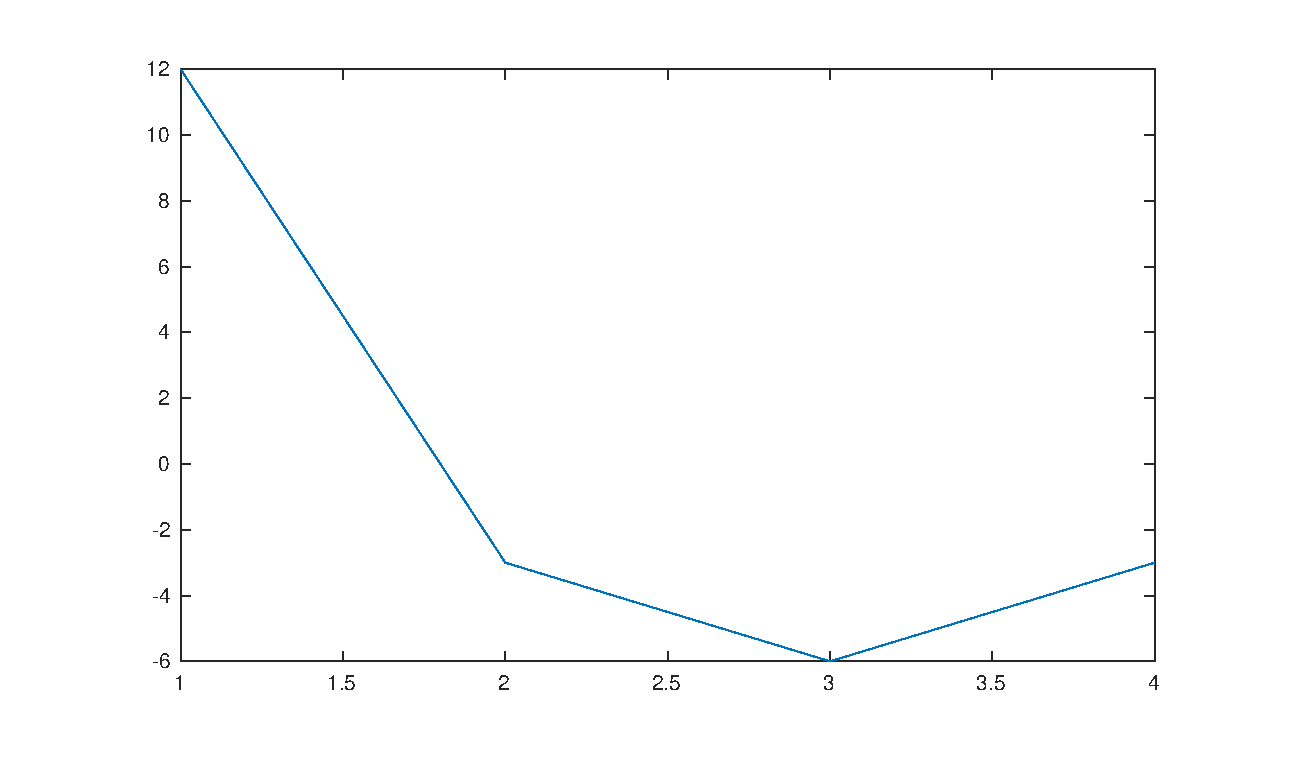
\includegraphics[width=0.7\textwidth]{task1.eps}
            \caption{Matlab plot of the real part of the \texttt{fft} of the
                discrete time series}
        \end{figure}
\end{enumerate}

\newpage
\ex{2}


\begin{enumerate}[label=\alph*)]
    \item test

    \item 
        \begin{align}
        \end{align}
\end{enumerate}




%% uncomment this if you need references. Edit the .bbl file with your references
%% and use "\cite{bibitem-label}" to cite
%\bibliography{template}

\end{document}

